\documentclass[conference, hidelinks]{IEEEtran}

\usepackage{subfigure}
\usepackage{hyperref}
\usepackage[pdftex]{graphicx}
\usepackage{lmodern}
\usepackage[utf8]{inputenc}
\usepackage{float} % laces the float at precisely the location in the LaTeX code
\usepackage{rotating} % Rotate figures or tabels into landscap mode
\usepackage{listings} % programming code syntax highlighting
\usepackage{subfigure}
\usepackage{amsmath} % Advanced math
\usepackage{hhline}
\usepackage{array}
\usepackage{caption}
\newcommand{\OneColumnWidth}{88.9mm}
\captionsetup[table]{skip=10pt}

\begin{document}
\title{Audio-based classification of Birds using Cased-Based Reasoning}

\author{
\IEEEauthorblockN{
  Alex Eskander Anis\IEEEauthorrefmark{1},
  Anna Enbom\IEEEauthorrefmark{2},
  Daniel Hedlund\IEEEauthorrefmark{3},
  Johan Söderlind Åström\IEEEauthorrefmark{4},
}

\IEEEauthorblockA{IDT Division,
MDH university --- Västerås, Sweden\\
Email:
\IEEEauthorrefmark{1}eas12003@student.mdh.se,
\IEEEauthorrefmark{2}jji15003@student.mdh.se,
\IEEEauthorrefmark{3}jam12003@student.mdh.se,\\
\IEEEauthorrefmark{4}sir15001@student.mdh.se}
}


\maketitle

\begin{abstract}
The pursuit of the perfect bird classifier is ongoing. Automated classifiers
can facilitate research such as ornithology and ecology, and prevent plane
crashes. In this paper we present how we used Case-based Reasoning to develop
an automated audio-based bird specie classifier. The case base was built out
of recordings from 8 different species. Frame division was used for higher
performance and we use periodogram as feature extraction method. Our project
resulted in a working application that can identify the specie of the bird
singing in the recording. Our goal was a high accuracy and a low footprint
which we achieved.
\end{abstract}

\begin{IEEEkeywords}
case-based reasoning; feature extraction; periodogram; spectrogram; classification;
audio;
\end{IEEEkeywords}

%\section{Introduction}
Bird song classification is not only useful for enthusiastic bird watchers.
It contributes to research fields such as ornithology and ecology[1], for
example conservatory planning [3] and the understanding of of how climate
change affects bird populations[1]. It is also useful for preventing plane
crashes caused by collisions with birds [3].

Singing serves different purposes for birds. For example identify individuals
and kinship, threaten rivals and choose partner [2]. Just like human speech,
bird song have a grammar and are built on syllables[3]. Some birds hide and
therefore sound is the only way for humans to know their precense.

Since automated bird classification can be more efficient and accurate than
manual, a lot of research has been done. One of the challenge is that the
recordings are nautrally noisy and can contain sound from many individuals
at the same time [2]. Extraction of useful features is crucial [3].

\section{Background and related work}
Robert Gubkar and Michal Kuba \cite{6566278}  from the university of Zilinia in Slovakia
conducted a study about comparision of audio features for elementary sound
based audio classification. They compared two sets of audio features for classification
of various sonds such as applause, crying, laugh, music, noise and speech.
The first set of features consist of mel-frequency ceptral coefficients together with
their first and seconds order time derivaties. The seconds set consists of line
spectral frequencies, spectral flux and zero crossing rate. Their test shows that
the second set of features were superior to classical MFCC coefficients for general
sound patter recognition and comparable for speech recognition.\\

Jijung Deng et. al.\cite{6138136} created a fingerprinting system based on spectral energy
structure of the audio signal. Audi fingerprint is a compact unique content-based
digital signature which is constructed based on features from the audio.
The used feature extraction method consists of filtering out the audio signal
to eliminate high-frequency noise and fourier-transform is applied to calculate
the energy of the subbands. Each subband energy is represented by 2 bits.
At last a sub-fingerprint of 2*(number of subbands-1) bits in binary form will
be produced from each frame of audio signal. The usage of inverted file
indexing technique combined with hash tables increased the speed of retrieval
process for the matching algorithm. Their preliminary experimental results
suggest that this method can work well in the application of broadcast
monitoring.\\


Identifying sounds using computers is not something new, the idea has been
around for a long time. So several different methods for this has been
developed, in this project Periodogram was used for feature extraction and
Case Based Reasoning was used for the decision making part.\\

This paper from 2014 \cite{danne1} instead decided to use Spectrogram combined with
Angular and Radial Transform (ART) for their feature extraction part. A
Spectrogram is a 3D representation of a sound file. This gives a lot of
potential features to extract but it is a lot harder to find and extract
these features than from a 2D graph. They solve this by using ART which is a
moment based image description method. This is then adopted in MPEG-7 as a
region-based shape descriptor, this gives an efficient way of expressing pixel
distribution in a 3D region. Essentially the 3D graph will instead be thought
of as a 3D image and this will allow the ART to analyze the shape and pixels,
this can be used to extract the features from the spectrogram. This is then
applied much in the same way we did with the sound file being analyzed with a
texture window creating overlapping frames where the features are extracted in
every frame. For their decision making they instead use Gaussian Mixture Models
(GMM) which is parametric probability density function. This method differs
from CBR in that you don't build a library of different cases and then compare
the current case to your library. Instead a GMM needs to be trained beforehand
and then uses weights to help in the decision making. In this case they used
Expectation-Maximization algorithms, each bird species will be represented as
a combination of Gaussian Component probability density functions.\\

Another paper that is not directly related to the work done in this project,
but is very important to the area of signal identification as a whole is \cite{1566472}.
Reconstruction of incomplete spectrograms for robust speech recognition, this
paper details a method for gaining a more robust recognition of speech when the
sound is corrupted by noise. When a signal is corrupted by noise some features
may be lost, normally a program would be trained with cases that have a similar
noise level. This methods ignore the lost features and use the remaining to
find the most likely match, this is by no means a foolproof method and this
only works with stationary noise. Non-stationary noise is even more error prone.
 This paper instead talks about the reconstruction of the corrupted data by
 estimating the missing components and after the data has been estimated the
 signal can be reconstructed and then classified with the speech recognition
 program. The paper details several different methods for reconstructing
 incomplete or corrupted spectrograms, either by treating the missing regions
 as completely unknown or treating them as unknown but bounded. Several
 different methods are introduced but the two most effective ones are cluster
 marginal reconstruction and covariance joint reconstruction.\\
 
 

Paper \cite{6497946} present a method to reduce the number of fingerprints or cases by increasing the fingerprint size which will improve memory consumtion and serch time.
"The proposed method uses the fingerprint extraction algorithm in time and frequency domains using wavelet transform. The audio signal was decomposed into 5-layer wavelet, and then calculated the energy distribution center, the energy of sub-band in wavelet domain, and the variance of wavelet coefficient. Finally, by using the results Calculated as the parameters of the audio fingerprints, the 8-bit fingerprint block per frame was generated" \cite{6497946}.

%\section{Method}
To make our bird recognition program we would essentially need two different parts. First a feature extraction method that can analyze and extract the desired features from a sound file of a bird singing. Secondly a decision making algorithm that can take the extracted features and classify which bird that sings in the sound file. The methods we choose for feature extraction was Periodogram (spectral density estimation) and CBR (Case Based Reasoning) was used for the decision making, we choose CBR specifically because it’s a tried and true decision making method. 

Periodogram
So for our project we used Periodogram to step through the sound file one frame at a time and then get the frequencies and corresponding amplitude in each frame. We did this using matlab. The sound file is first loaded into the program and the frame size is set depending on the length of the sound file, the step size is preset. After that the program basically uses the “Periodogram” function already present in matlab to create a periodogram of the frame illustrated in Fig.1. After that the “Findpeak” function is used to find the two highest peaks in the frame see Fig.2, this corresponds to the two frequencies that have the highest amplitude. One of the biggest reasons we choose Periodogram for our feature extraction was because of the ease of which you can find peaks in a two dimensional graph. This information along with the mean value and standard deviation is stored in an array. This is then done for the next frame and so on until the entire sound file has been analyzed as can be seen in Fig.3. This array is then exported as a csv file that will be used in the CBR program. To create the case library for the CBR several sound files of different birds are analyzed and exported into csv files.

CBR
The files created with the Periodogram are then put where the CBR can find them. So when the CBR runs you have to tell it which of the frames you want in to test, the program will then compare the features in this frame to the cases that are already in the library. The features which are relevant for our program are the two frequencies with the highest amplitude, in this case it the decibel value is the amplitude. The program will use the KNN (K-nearest neighbour) algorithm to determine which bird made the sound. We have tried several different similarity functions but the one we decided to use in our final program was Euclidian distance simply because it gave us the best performance. Only two features is usually not enough to get a robust algorithm, so the program will need another frame from the same source and will also run this through the KNN algorithm. The results from the two frames are then compared and the the class with the most neighbours from both of the frames is chosen see Fig.4.

%\input{evaluation.tex}
\section{Results}
The development of the bird classifier using cased-based reasoning has
been successful in many ways. The final version met all the initial requirements
stated at the beginning of the project and the code has a low footprint while
providing an adequate performance. The leave-one-out-bird cross-validation method has been used
for the validation of the CBR. In details, for validation of the CBR another audio recording
of a bluethroat bird (called bluethroat2) has been added and validated against the database.
Since the database already includes features from bluethroat, a valid classification is expected.

In Figure~\ref{fig:results1} and other figures in this section, we see number of matches over number of
neighbours when comparing 137 samples or 4 seconds of Bluethroat2 against the database. Different figures
represent different weight and distance function configurations.


\begin{figure}[htp]
    \subfloat[Canberra. \fontfamily{qcr}\selectfont \newline 1.0 * FFT Peak 1]{
      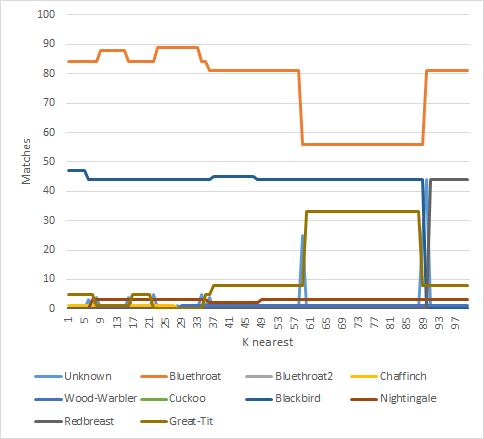
\includegraphics[clip,width=0.4\columnwidth]{eval-canberra-0_0-0_0-1_0-0_0-0_0-0_0-0_0-0_0}
    }
    ~
    \subfloat[Canberra. \fontfamily{qcr}\selectfont \newline 1.0 * FFT Peak 1 \newline 1.0 * FFT Peak 1 Delta]{
      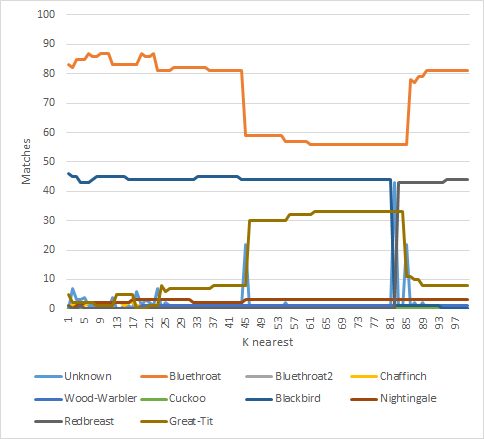
\includegraphics[clip,width=0.4\columnwidth]{eval-canberra-0_0-0_0-1_0-0_0-1_0-0_0-0_0-0_0}
    }
    \caption{Comparing 137 samples or 4 seconds of Bluethroat2 against the database. X-axis is the number of nearest neighbours (the k value) and Y-axis is number of matches for each class of bird.
    This shows adding FFT Peak 1 Delta does not yield significantly better result.  }
    \label{fig:results1}
\end{figure}

\begin{figure}[htp]

  \subfloat[Canberra. \fontfamily{qcr}\selectfont \newline 0.1 * FFT Area Delta. \newline 1.0 * FFT Peak 1 Delta]{
    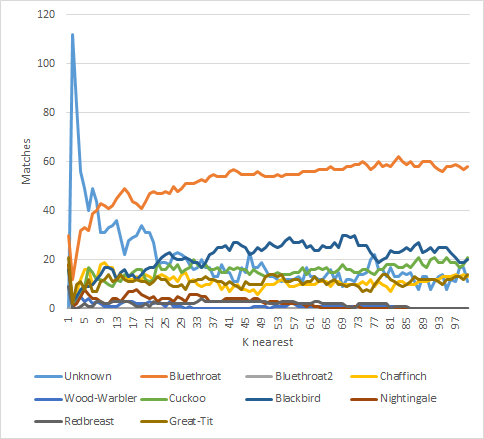
\includegraphics[clip,width=0.4\columnwidth]{eval-canberra-0_0-0_1-0_0-0_0-1_0-0_0-0_0-0_0}
  }
  ~
  \subfloat[Canberra. \fontfamily{qcr}\selectfont \newline 1.0 * FFT Area Delta. \newline 1.0 * FFT Peak 1 Delta]{
    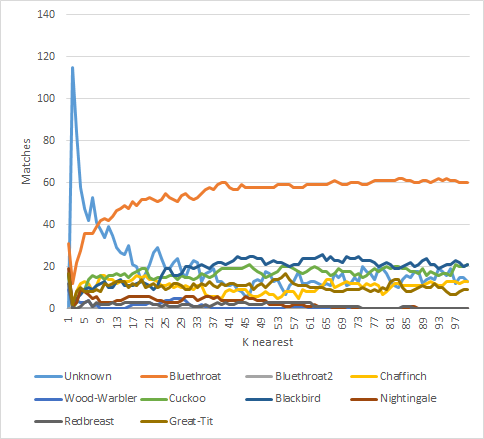
\includegraphics[clip,width=0.4\columnwidth]{eval-canberra-0_0-1_0-0_0-0_0-1_0-0_0-0_0-0_0}
  }
    \caption{This shows a good combination of weights. Note that FFT Peak 1 Delta is necessary.}
    \label{fig:results2}
\end{figure}



\begin{figure}[htp]
    \subfloat[Canberra. \fontfamily{qcr}\selectfont \newline 1.0 * FFT Peak 1 Delta]{
      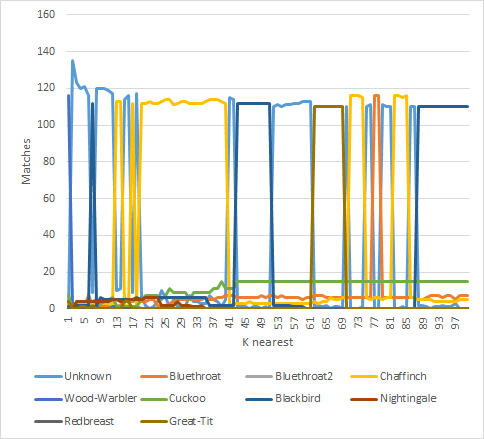
\includegraphics[clip,width=0.4\columnwidth]{eval-canberra-0_0-0_0-0_0-0_0-1_0-0_0-0_0-0_0}
    }
    \caption{Note that FFT Peak 1 Delta alone does not yield acceptable result.}
    \label{fig:results3}
\end{figure}




\begin{figure}[htp]
    \subfloat[Canberra. \fontfamily{qcr}\selectfont \newline 1.0 * FFT Area Delta \newline 0.1 * FFT Peak 1]{
      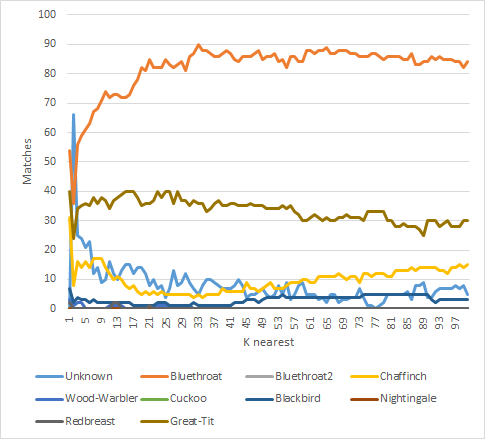
\includegraphics[clip,width=0.4\columnwidth]{eval-canberra-0_0-1_0-0_1-0_1-1_0-0_0-0_0-0_0}
    }
    ~
    \subfloat[Canberra. \fontfamily{qcr}\selectfont \newline 1.0 * FFT Area Delta \newline 1.0 * FFT Peak 1]{
      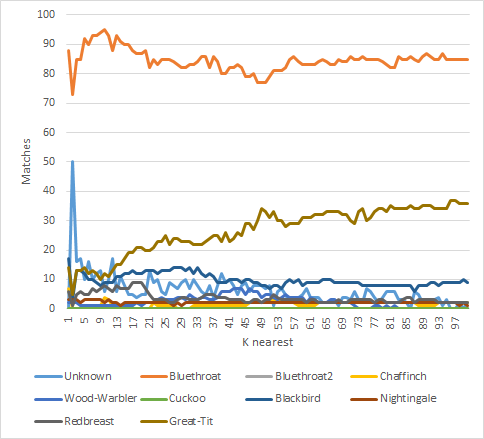
\includegraphics[clip,width=0.4\columnwidth]{eval-canberra-0_0-1_0-1_0-0_0-0_0-0_0-0_0-0_0}
    }

    \subfloat[Canberra. \fontfamily{qcr}\selectfont \newline 1.0 * FFT Area Delta \newline 1.0 * FFT Peak 1  \newline 1.0 * Peak 1 Delta]{
      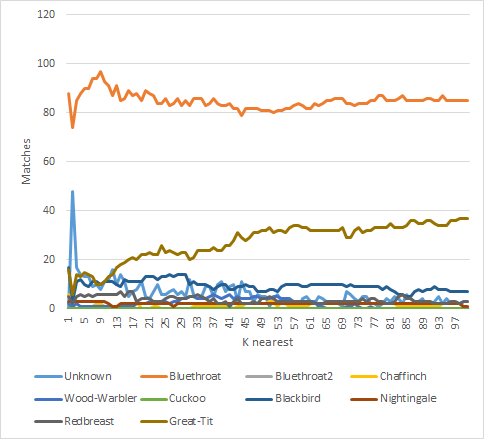
\includegraphics[clip,width=0.4\columnwidth]{eval-canberra-0_0-1_0-1_0-0_0-1_0-0_0-0_0-0_0}
    }
    \caption{}
    \label{fig:results4}
\end{figure}


\begin{figure}[htp]
    \subfloat[Canberra. \fontfamily{qcr}\selectfont \newline 1.0 * FFT Area \newline 1.0 * FFT Area Delta \newline 1.0 * Peak 1 \newline 1.0 * Peak 2 \newline 1.0 * Peak 1 Delta]{
       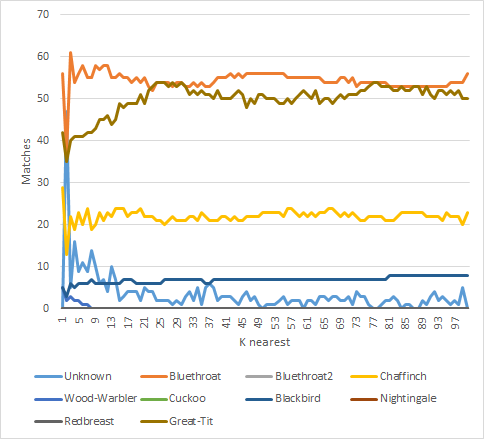
\includegraphics[clip,width=0.4\columnwidth]{eval-canberra-1_0-1_0-1_0-1_0-1_0-0_0-0_0-0_0}
    }
    ~
    \subfloat[Euclidean. \fontfamily{qcr}\selectfont \newline 1.0 * FFT Area \newline 1.0 * FFT Area Delta \newline 1.0 * Peak 1 \newline 1.0 * Peak 2 \newline 1.0 * Peak 1 Delta]{
      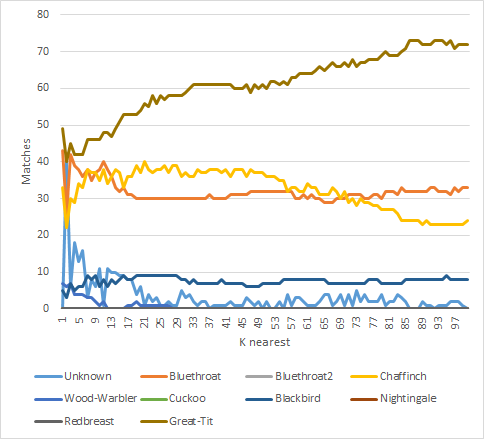
\includegraphics[clip,width=0.4\columnwidth]{eval-euclidean-1_0-1_0-1_0-1_0-1_0-0_0-0_0-0_0}
    }

    \subfloat[Euclidean. \fontfamily{qcr}\selectfont \newline 1.0 * FFT Area \newline 1.0 * FFT Area Delta \newline 1.0 * Peak 1 \newline 1.0 * Peak 2 \newline 1.0 * Peak 1 Delta \newline 1.0 * Mean \newline 1.0 * STD]{
      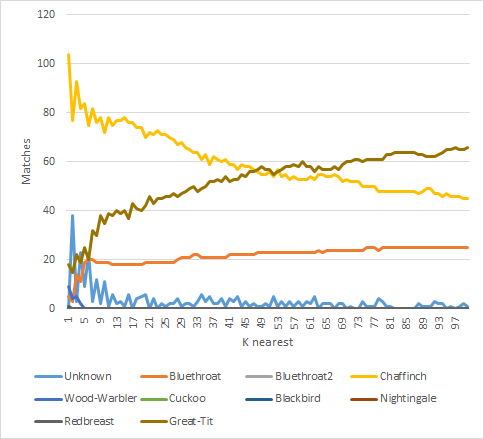
\includegraphics[clip,width=0.4\columnwidth]{eval-euclidean-1_0-1_0-1_0-1_0-1_0-1_0-1_0-0_0}
    }
    \caption{}
    \label{fig:results5}
\end{figure}

\begin{figure}[htp]
    \subfloat[Euclidean. \fontfamily{qcr}\selectfont \newline 1.0 * FFT Area \newline 1.0 * FFT Area Delta \newline 1.0 * Peak 1 \newline 1.0 * Peak 2 \newline 1.0 * Peak 1 Delta \newline 1.0 * Mean \newline 1.0 * STD \newline 1.0 * ZCR]{
      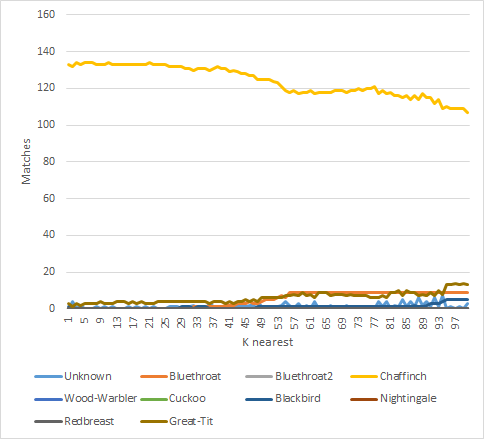
\includegraphics[clip,width=0.4\columnwidth]{eval-euclidean-1_0-1_0-1_0-1_0-1_0-1_0-1_0-1_0}
    }
    ~
    \subfloat[Canberra. \fontfamily{qcr}\selectfont \newline 1.0 * FFT Area \newline 1.0 * FFT Area Delta \newline 1.0 * Peak 1 \newline 1.0 * Peak 2 \newline 1.0 * Peak 1 Delta \newline 1.0 * Mean \newline 1.0 * STD \newline 1.0 * ZCR]{
      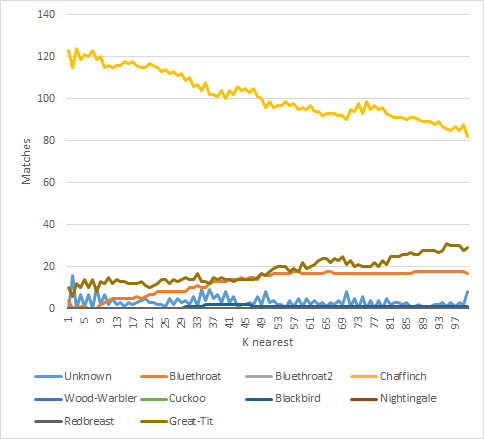
\includegraphics[clip,width=0.4\columnwidth]{eval-canberra-1_0-1_0-1_0-1_0-1_0-1_0-1_0-1_0}
    }

    \subfloat[Manhattan. \fontfamily{qcr}\selectfont \newline 1.0 * FFT Area \newline 1.0 * FFT Area Delta \newline 1.0 * Peak 1 \newline 1.0 * Peak 2 \newline 1.0 * Peak 1 Delta]{
      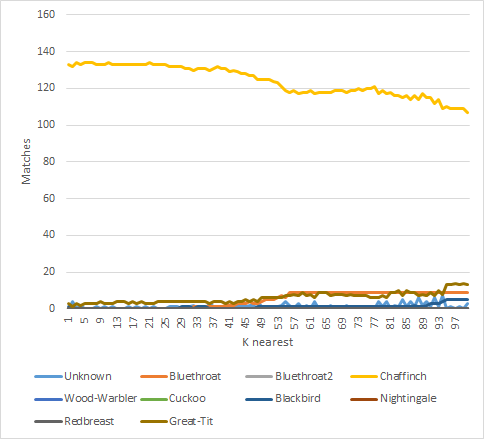
\includegraphics[clip,width=0.4\columnwidth]{eval-manhattan-1_0-1_0-1_0-1_0-1_0-0_0-0_0-0_0}
    }
    \caption{As we can see these outputs mostly Chaffinch bird which is the wrong one. Using all features does not work.}
    \label{fig:results6}
\end{figure}

The test has showed that it is possable to classify a noisy, different audio strength Bluethroat2 compared to a database with no noize and high quality audio sounded birds.

The tests shows that using Euclidian and Manhattan distance does not yield to accurate results.
The most accurate result were achieved by using the Canberra distance function with different
weight configurations. List of proposed configurations which yield high accuracy include:
\begin{itemize}
  \item Configuration 1: Canberra, 1.0 * FFT Peak 1 Delta, 1.0 * FFT Area Delta.
  \item Configuration 2: Canberra, 1.0 * FFT Peak 1.
  \item Configuration 3: Canberra, 1.0 * FFT Peak 1, 1.0 * FFT Area Delta.
  \item Configuration 4: Canberra, 1.0 * FFT Area Delta, 0.2 * FFT Peak 1, 0.1 * FFT Peak 2, 1.0 * FFT Peak 1 Delta
\end{itemize}

These configurations are found by trial and error and therefore, better configurations may exist.

\section{Discussion}
Configuration number four is currently the best mean accuracy over K from 1 to 100.
Some features can not act alone while others, for example FFT Peak 1 can produce a high accuracy.
When FFT Peak 1 is combined with other features the result will improve if the
weight is decreased for FFT Peak 1. This conclude that that a dominating feature
like FFT Peak 1 may not be that important. It is important not to get biased for
a feature even if that feature alone gives better result than the others.

\section{Summary and conclusions}
The developed classifier met all the requirements which were validated
by the various tests performed. Audio files of eight different birds has been
acquired while the birds are singing. A moving window
with a predefined boundaries scans the signal in the time domain and a tranformation
from the time-domain to frequency domain has been conducted in order to extract features.
The two frequencies with the highest amplutide have been extracted for each frame.
These two features together with the class constitute the database for CBR.

The CBR written in the Ada programming language uses the K nearest approach to
find the most similar cases and the user can specify the similarity formula with ease.
The leave-one-out cross-validation method has been used for the validation of the CBR system.

A natural evolution of this classifier would be to use more appropriate features
and adjusting the feature weights accordingly. Also remvoing duplicate data from
the the database would increase the precision of the system and when that happens
the user can test for classification of other animals such as whales or dogs.

With higher reliability, this system could be used for people with hearing impairment
in order to hear the sound of different subjects by using vibration motors. 

\section{Acknowledgments}
The authors wish to express their gratitude to our customer, Kristian Sandström
(Principal Scientist, ABB) for providing us the opportunity to participate in
the real-time operating system development project. Further, the authors would
like to express their gratitude to our project managers, Moris Behnam and Nils
Müllner, for the guidance provided to us during the weekly project review
meetings.  And last but not the least, the authors would like to express their
gratitude to our technical experts, Mohammad Ashjaei and Nesredin Mahmud, for
resolving our various technical questions.

%\bibliographystyle{ieeetran}
%\bibliography{bibliography}
\end{document}
